\section{Evaluation}

\label{sec_impl_evaluation}

%\begin{itemize}
%  \item Geeignete Stelle zum Eingriff in den Datenfluss zwischen Logdatenquelle und SIEM-System
%  \item Parameterabhängige Generierung eindeutiger, aber in gewissem Rahmen verknüpfbarer Pseudonyme
%  \item Sicherer, verteilter Einsatz eines anpassbaren kryptographischen Schwellwertschemas -- vorzugsweise mit verteilter Schlüsselgenerierung
%  \item Geeignete Benutzerinteraktion mit dem System an notwendigen Stellen
%  \item Erweiterbarkeit um unbekannte Datenquellen
%  \item Erweiterbarkeit um weitere Datenschutztechniken
%\end{itemize}

Grundsätzlich konnten die in Abschnitt \ref{sec_impl_requirements} aufgestellten Anforderungen in der Implementierung des Prototypen erfüllt werden. Mit der Entwicklung eines Log-Proxies wurde eine geeignete Stelle für den Eingriff in den Logdatenfluss gewählt. Die Zeit-und Nutzungsabhängige Generierung eindeutiger Pseudonyme wurde ebenso umgesetzt wie die Implementierung des ausgewählten Schwellwertschemas -- vorerst allerdings nur mit zentraler Schlüsselgenerierung. Die benötigten Parameter können während des Setup-Vorgangs über ein Webinterface gesetzt werden. Dieses ermöglicht auch die Erstellung von Anfragen zur Aufdeckung eines Pseudonymhalters. Besitzer eines Shares können diese Anfragen bearbeiten oder ablehnen (momentan allerdings noch eher unkomfortabel über eine Konsolenanwendung). Der entwickelte Log-Proxy ist einfach um weitere Datenschutztechniken und Datenquellen erweiterbar.

In dem Prototypen bleiben allerdings auch noch einige Angriffsmöglichkeiten offen, die im nächsten Abschnitt dargestellt werden. Betrachtungen zur Performanz der entwickelten Lösung werden in dem darauf folgenden Abschnitt angestellt.

\subsection{Angriffsmöglichkeiten}


%- Zentrale Schlüsselgenerierung (Verweis auf state-distributed)

\textbf{Zentrale Schlüsselgenerierung}

Ein bereits in Abschnitt \ref{subsec_impl_requirements_threshold} betonter Punkt ist die Präferenz von verteilter gegenüber der zentralen Schlüsselgenerierung. In dem entwickelten Prototypen wurde jedoch aus Zeitgründen bisher nur die zentrale Schlüsselgenerierung umgesetzt. Dies ermöglicht einem Angreifer mit (legitimen oder nicht legitimen) Zugriff auf den Pseudo-Service während der Schlüsselgenerierung den in Abschnitt \ref{subsec_impl_requirements_attackermodel} beschriebenen Angriff zur beliebigen Entschlüsselung von Pseudonymzuordnungen. Abhilfe würde ein Schema -- wie das in Abschnitt \ref{sec_state_threshold_distributed} beschriebene -- schaffen.

%- Krypto nicht von Kryptographen überprüft (Sidechannel, ...)

\textbf{Nicht überprüfte kryptographische Funktionen}

Die Bibliotheksfunktionen des kryptographischen Schwellwertschemas wurden nach bestem Wissen und Gewissen umgesetzt. Trotzdem wurden sie bisher nicht von erfahrenen Kryptographen überprüft und können daher eine Vielzahl von Schwächen und Angriffsmöglichkeiten aufweisen. Die Nutzung einer quelloffenen und vielfach überprüften Bibliothek wäre wünschenswert, aber wie in Abschnitt \ref{sec_state_threshold_existing_impl} beschrieben, wurde eine solche Bibliothek nicht gefunden.

%- Scheme leakt Nachrichtenlänge als Vielfaches der Blocklänge -> Paddingscheme?

\textbf{Schlüsseltexte offenbaren Klartextlänge}

Eine Eigenschaft des entwickelten hybriden Kryptoschemas kann dazu führen, dass trotz der Verschlüsselung auf den Halter eines Pseudonyms geschlossen werden kann. Bei dem verwendeten symmetrischen Verschlüsselungsalgorithmus Salsa20 handelt es sich um eine Stromchiffre. Hierdurch hat der Schlüsseltext, der in der Datenbank für ein Pseudonym gespeichert wird, genau die gleiche Länge wie der Klartext. Unterscheiden sich die Klartexte (beispielsweise Benutzernamen) in Ihrer Länge, so kann durch Vergleich dieser Längen auf den Pseudonymhalter geschlossen werden.  Dieser Angriff erfordert Zugriff auf den Inhalt der Datenbank des Pseudo-Service.\\
Dieses Problem lässt sich durch Padding beheben, das alle Klartexte auf die gleiche Länge bringt. Die konkrete Umsetzung ist allerdings abhängig von dem Wertebereich der eintreffenden Daten.

%- Reidentification-Problem (siehe auch Lundin 4.3)

\textbf{Anwendung von Hintergrundwissen}

In \cite{lundin1999privacy} wird das Problem der Identifikation eines Pseudonymhalters durch die Anwendung von Hintergrundwissen wie Kenntnis über normales Nutzerverhalten dargestellt. Dies ist auch in dem in dieser Arbeit entwickelten System der Fall wie bereits in Abschnitt \ref{subsec_impl_requirements_attackermodel} erwähnt. Dieser Angriff lässt sich aus Sicht des Autors nicht vollständig verhindern, da Beobachtungen in der realen Welt nicht zu vermeiden sind.
Regelmäßige, parameterabhängige Pseudonymwechsel, wie sie implementiert wurden, sollten diesen Angriff jedoch in seinen Auswirkungen beschränken.



\subsection{Performanz}

- Zeitmessungen für einzelne Systemfunktionen

- Performance bzw. Auswirkungen der Nutzung (theoretische Rechenlast, Zeit-/Lastmessung, zusätzlicher Speicherbedarf, ...)


- Bar Chart Times per Key size
\begin{figure}[]
    \centering
    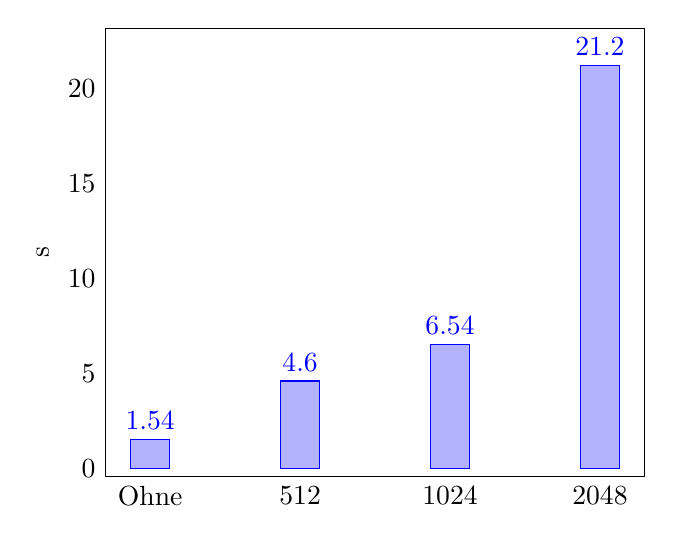
\begin{tikzpicture}
      \begin{axis}[%title  = ,
        ybar,
        bar width=.5cm,
        ylabel={s},
        %y axis line style = { opacity = 0 },
        %axis x line       = none,
        tickwidth         = 0pt,
        symbolic x coords = {Ohne, 512, 1024, 2048},
        xtick=data,
        nodes near coords,
      ]
      \addplot coordinates { 
        (Ohne, 1.54)
        (512, 4.60)
        (1024, 6.54)
        (2048, 21.20) 
      };
      \end{axis}
    \end{tikzpicture}
    \caption{Dauer der Bearbeitung von 100 Lognachrichten in Sekunden.}
    \label{fig:eval_barchart}
\end{figure}

\begin{figure}[]
    \centering
    \begin{tikzpicture}
    %512
    \pie[
       rotate = 90, 
       radius = 2,
       color = {blue!20, green!40, red!60},
       %text = legend,
       after number={},
     ] {
         97/,
         2/, 
         1/
     }
    
    %1024
     \pie[
        pos={4.5,0},
        rotate = 90, 
        radius = 2,
        color = {blue!20, green!40, red!60},
        %text = legend,
        after number={},
     ] {
         93/,
         6/, 
         1/
     }
    %2048
     \pie[
         pos={9,0},
          rotate = 90, 
          radius = 2,
          color = {blue!20, green!40, red!60},
          text = legend,
          after number={},
      ] {
          63/Pseudonym,
          36/Schwellwert, 
          1/Hash
      }
    \end{tikzpicture}
    \caption{Zeitlicher Anteil der verschiedenen Berechnungen im Pseudonymisierungs-Plugin bei  Schlüssellängen von 512 Bit (links), 1024 Bit (Mitte) und 2048 Bit (rechts).}
    \label{fig:eval_piecharts}
\end{figure}



- Pie Chart Times per Computational part

- Not  deployed in a standard way (uWSGI, Apache, ...)
- Crashes of PostgresSQl database driver
- Unreliability of UDP